% Created 2016-11-14 Mon 03:07
% Intended LaTeX compiler: xelatex
\documentclass[presentation]{beamer}
\usepackage{graphicx}
\usepackage{grffile}
\usepackage{longtable}
\usepackage{wrapfig}
\usepackage{rotating}
\usepackage[normalem]{ulem}
\usepackage{amsmath}
\usepackage{textcomp}
\usepackage{amssymb}
\usepackage{capt-of}
\usepackage{hyperref}
\usepackage{minted}
\usetheme{default}
\author{Paul M. Magwene}
\date{Fall 2016}
\title{Comparing samples using \(t\)-tests}
\setlength{\parskip}{0.75\baselineskip} 

%% Theme Settings
\useinnertheme[shadow,outline]{chamfered} 
\usecolortheme{beaver}
\beamertemplatenavigationsymbolsempty

%% Font Settings
\usepackage[no-math]{fontspec}
\defaultfontfeatures{Scale = MatchLowercase}
\setmainfont{Lucida Bright OT}
\setsansfont{Lucida Sans OT}
\setmonofont{PragmataPro}
\setmathrm{Lucida Bright Math OT}
\setmathsf{Lucida Sans OT}
\usefonttheme{structurebold}

%% Minted settings
\usepackage[breaklines]{minted}
\usepackage{mdframed}
\surroundwithmdframed[leftmargin=3em,backgroundcolor=gray!5]{minted}

\definecolor{links}{HTML}{2A1B81}
\hypersetup{colorlinks,linkcolor=,urlcolor=magenta}

\hypersetup{
 pdfauthor={Paul M. Magwene},
 pdftitle={Comparing samples using \(t\)-tests},
 pdfkeywords={},
 pdfsubject={},
 pdfcreator={Emacs 25.1.1 (Org mode 9.0)}, 
 pdflang={English}}
\begin{document}

\maketitle

\begin{frame}[label={sec:org7ba87ad}]{The \(t\)-distribution}
\begin{itemize}
\item When working with small samples, and the population standard deviation is unknown (usually the case), the uncertainty of the standard error estimate is addressed by using the \alert{\alert{t-distribution}}

\item This distribution also has a bell shape, but its tails are thicker than the normal model’s.

\item Therefore observations are more likely to fall beyond two SDs from the mean than under the normal distribution.

\item These extra thick tails are helpful for resolving our problem with a less reliable estimate the standard error (since \(n\) is small)
\end{itemize}

\begin{center}
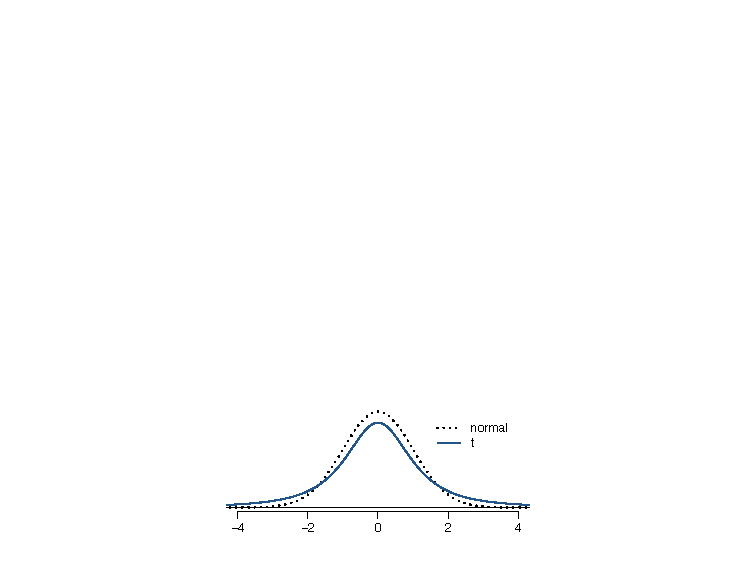
\includegraphics[height=0.30\textheight]{fig-t-vs-normal.pdf}
\end{center}


\credit{Credit: OpenIntro Stats, 3rd ed.}
\end{frame}


\begin{frame}[label={sec:orgb69da39}]{The \(t\)-distribution, cont.}
\begin{itemize}
\item Centered at zero, like the standard normal distribution

\item Has a single parameter, \alert{\alert{degrees of freedom}} (\(df\))
\end{itemize}

\begin{center}
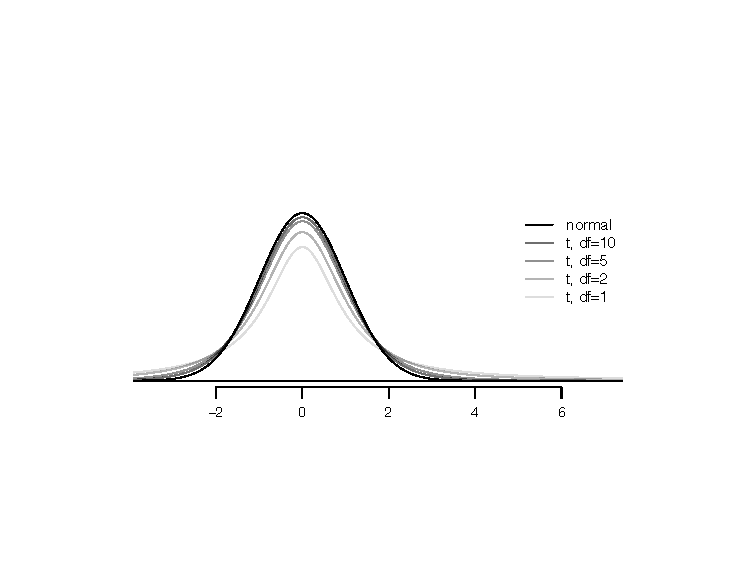
\includegraphics[height=0.40\textheight]{fig-tdistn-df.pdf}
\end{center}

What happens to the shape of the distribution as the degrees of freedom increases?

\credit{Credit: OpenIntro Stats, 3rd ed.}
\end{frame}

\begin{frame}[label={sec:orge122282}]{One sample inference using the \(t\)-distribution}
\begin{itemize}
\item If \(n < 30\), sample means follow a \(t\)-distribution with \(SE = \frac{s}{\sqrt{n}}\) and \(df = n - 1\)
\item Conditions:
\begin{itemize}
\item independence of observations (random sample, \(n\) < 10\% of population)
\item No extreme skew
\end{itemize}
\item Confidence interval for mean:
\end{itemize}
\[
\text{point estimate} \pm t_{df}^{\star} \times SE
\]
\begin{itemize}
\item Hypothesis testing, test statistic:
\end{itemize}
\[
T = \frac{\text{point estimate} - \text{null value}}{SE}
\]

\credit{Credit: OpenIntro Stats, 3rd ed.}
\end{frame}

\begin{frame}[fragile,label={sec:org79c1e5d}]{One-sample t-test, example}
 You treat a sample of mice with a drug, X, and measure the expression of the gene YFG1 following treatment. For a sample of five mice you observe the following expression values:

\begin{itemize}
\item X = \{11.25, 10.5, 12, 11.75, 10\}
\end{itemize}

This data set can be downloaded from the class wiki as the file \texttt{gene-expression-1sample.csv}
\end{frame}

\begin{frame}[label={sec:org1a6936c}]{One-sample t-test, relevant distributions and comparisons}
\begin{center}
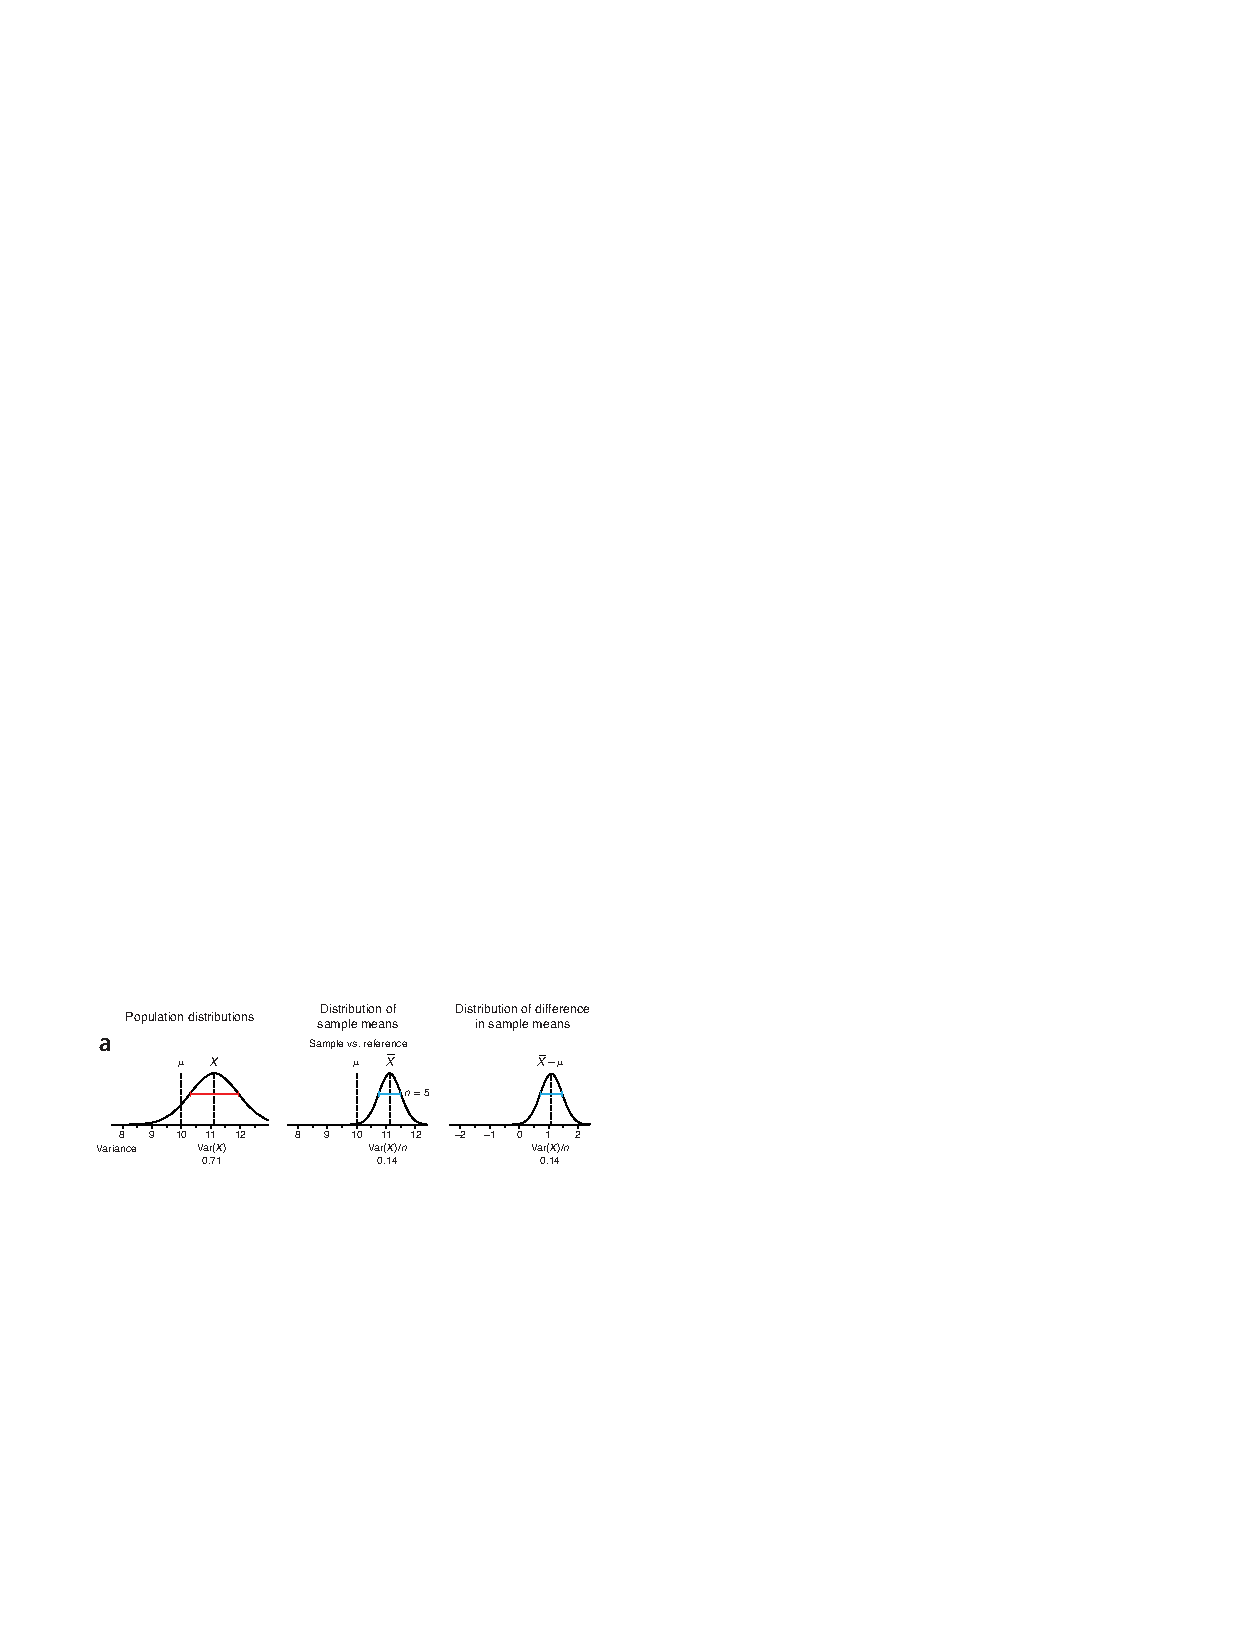
\includegraphics[height=0.33\textheight]{fig-onesample-distns.pdf}
\end{center}


\begin{center}
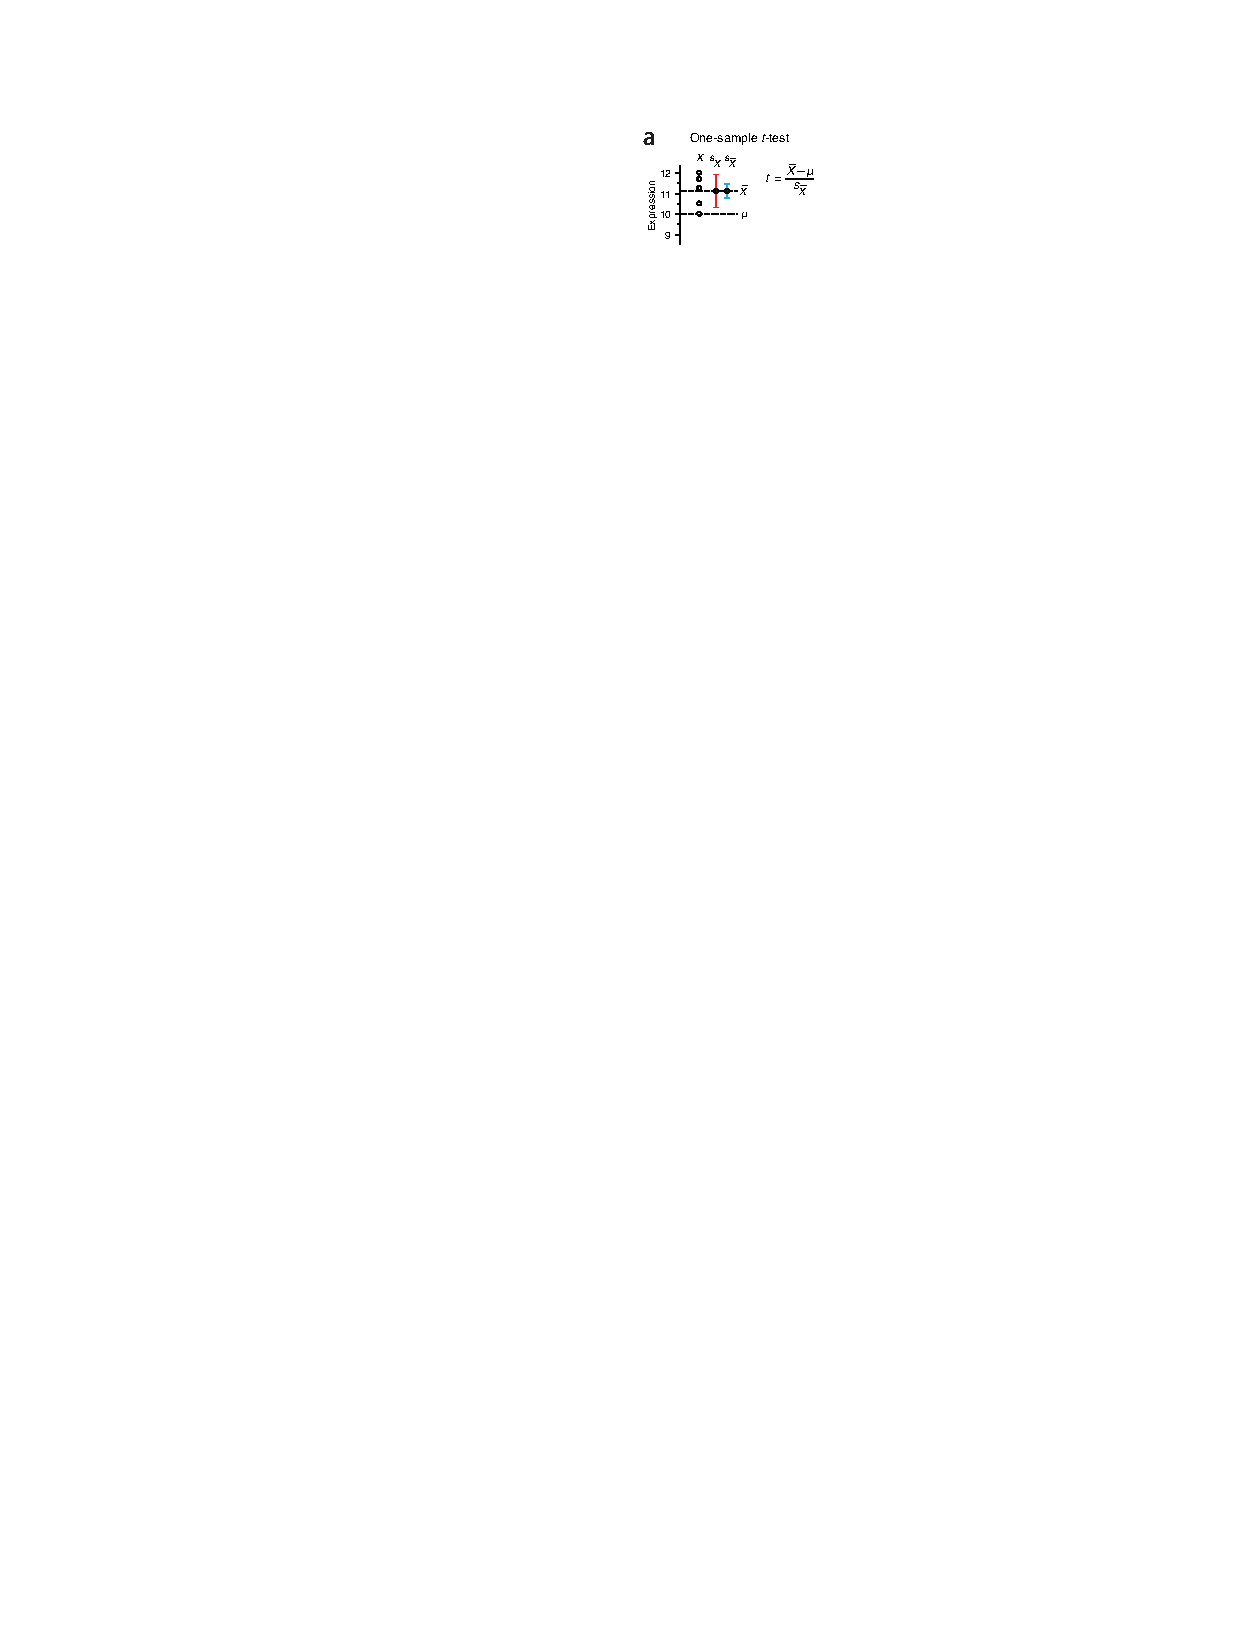
\includegraphics[height=0.30\textheight]{fig-onesample-ttest.pdf}
\end{center}


\credit{Image credit: Krzywinski \& Altman 2014}
\end{frame}

\begin{frame}[fragile,label={sec:org482fa1e}]{Hands-on, one-sample t-test}
 You have established from previous studies that the expression level of YFG1 in control mice is 10.  You wish to determine whether the average expression of YFG1 in mice treated with drug X differs from control mice.

\begin{enumerate}
\item Write down an appropriate null and alternative hypothesis.
\item Calculate 95\% confidence intervals for the mean expression of YFG1 in the sample data set
\item Calculate the test statistic \(T\)
\item Calculate a p-value giving the probability that you'd find an average expression value at least as extreme as that observed, if the null hypothesis was true
\end{enumerate}

Hint: Recall the \texttt{dt}, \texttt{pt}, \texttt{qt} and \texttt{rt} functions for working with the \(t\)-distribution
\end{frame}


\begin{frame}[fragile,label={sec:org59aafcc}]{t-tests in R}
 The R function \texttt{t.test} makes it easy to calculate one- and two-sample t-tests

\begin{enumerate}
\item Read the help documentation on \texttt{t.test}
\item Carry out a one-sample t-test for the gene expression data set, using the null hypothesis that average gene expression for YFG1 is 10
\item Do the results given by \texttt{t.test} correspond to the your ``by hand'' calculations from the previous exercise?  If not, go back and figure out where your previous calculations went awry.
\end{enumerate}
\end{frame}


\begin{frame}[label={sec:org2412b80}]{Two-sample t-test}
The two-sample t-test is used to determine if two populations, represented by observed samples, have equal means.


Test statistic:
\[
T = \frac{\overline{X_1} - \overline{X_2}}{\sqrt{\frac{s_1^2}{n_1} + \frac{s_2^2}{n_2}}} 
\]
\end{frame}


\begin{frame}[fragile,label={sec:org4707751}]{Two-sample t-tests, example}
 You treat samples of mice with two drugs, X and Y.  We want to know if the two drugs have the same average effect on expression of the gene YFG1. The measurements of YFG1 in samples treated with X and Y are as follows: 


\begin{itemize}
\item X = \{11.25, 10.5, 12, 11.75, 10\}
\item Y = \{8.75, 10, 11, 9.75, 10.5\}
\end{itemize}

This data set is available on the course wiki as \texttt{gene-expression-2sample.csv}
\end{frame}


\begin{frame}[label={sec:org0b9d4d0}]{Two-sample t-tests, relevant distributions and comparisons}
\begin{center}
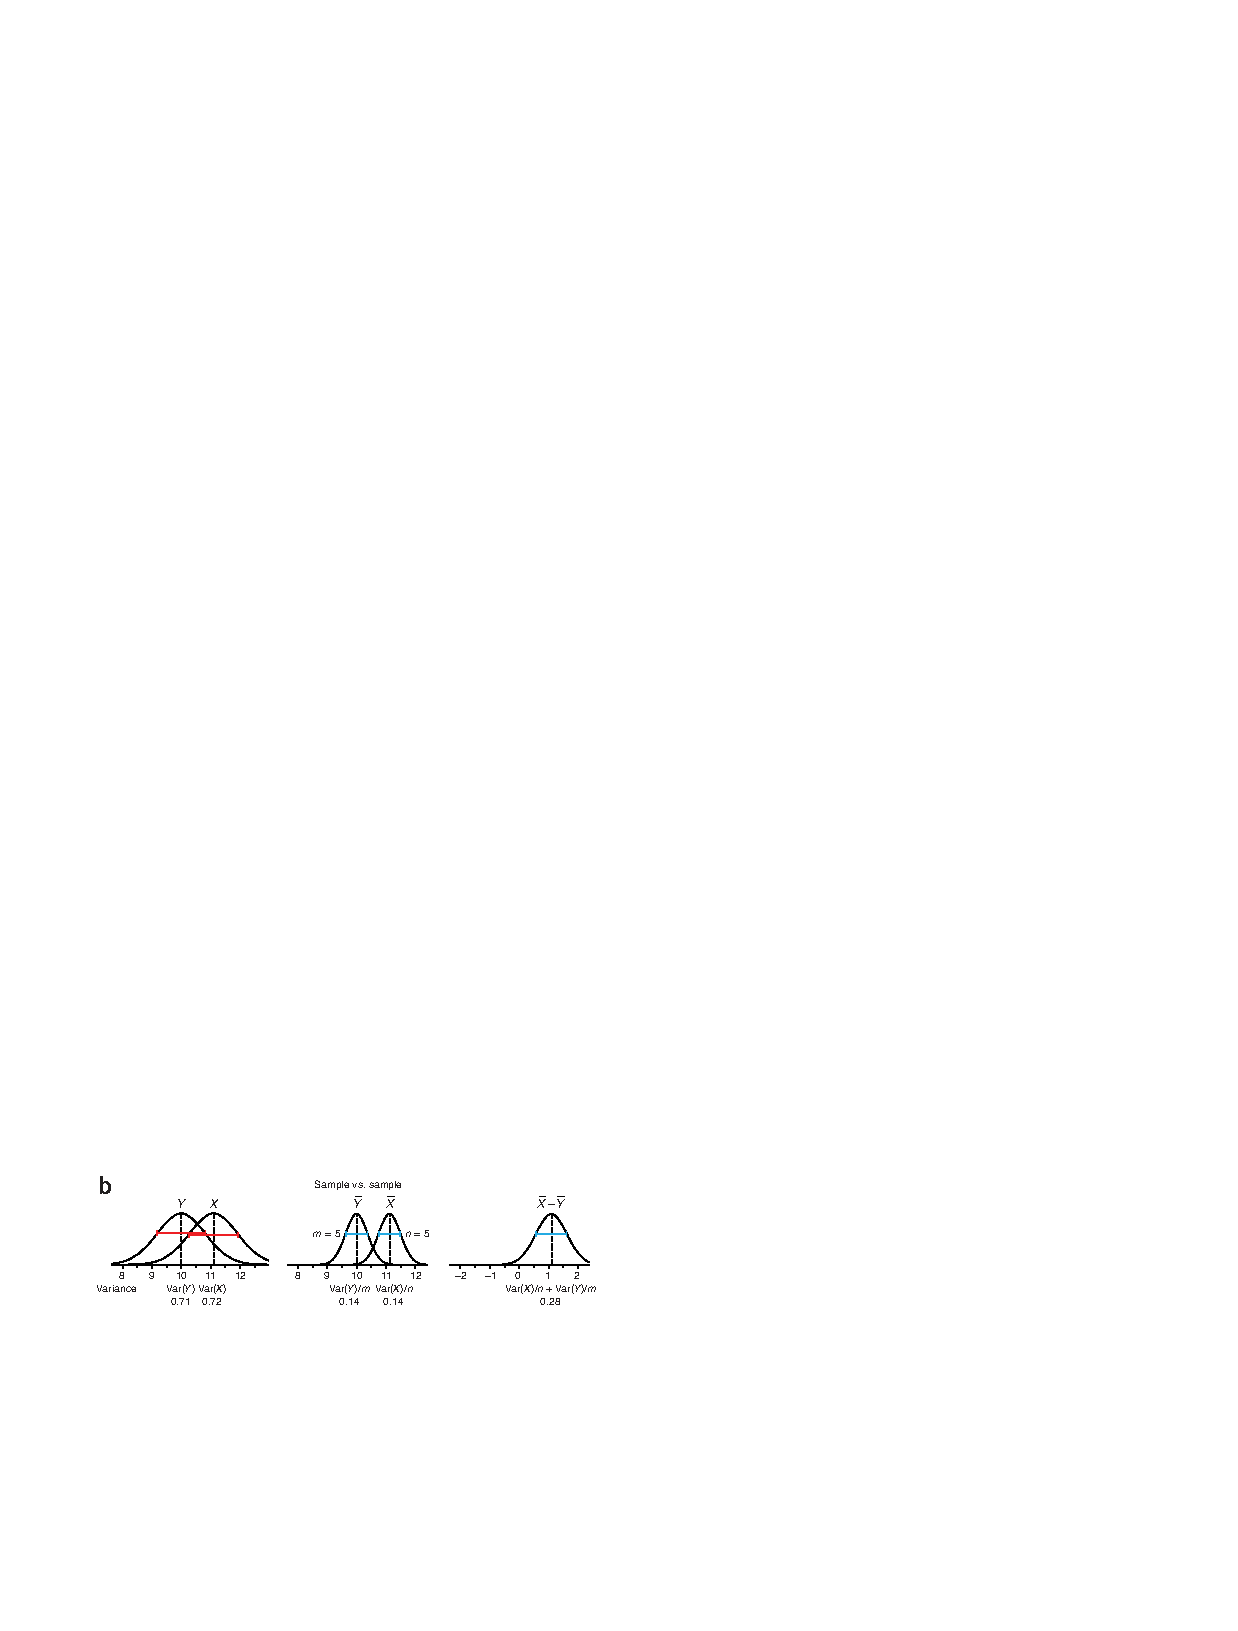
\includegraphics[height=0.33\textheight]{fig-twosample-distns.pdf}
\end{center}


\begin{center}
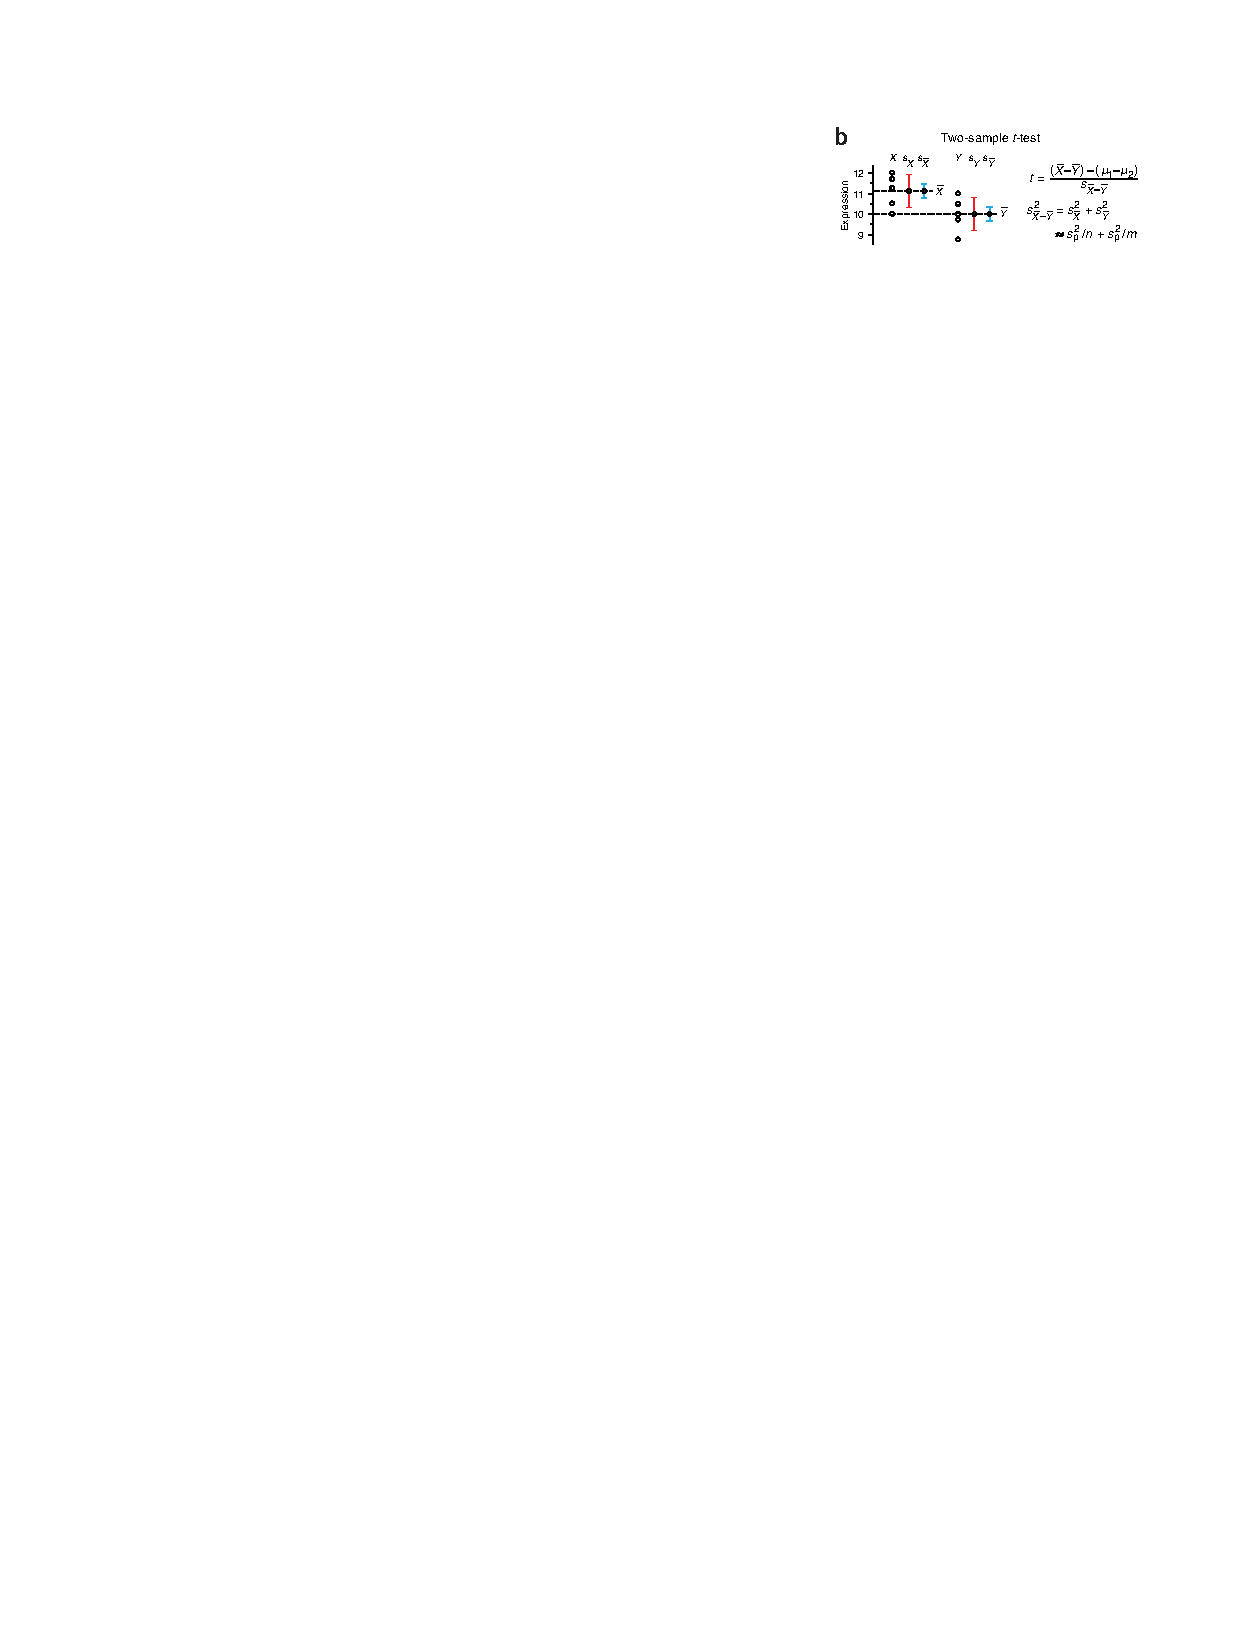
\includegraphics[height=0.30\textheight]{fig-twosample-ttest.pdf}
\end{center}

\credit{Image credit: Krzywinski \& Altman 2014}
\end{frame}

\begin{frame}[fragile,label={sec:org01d311b}]{Hands-on, two-sample t-tests in R}
 The \texttt{t.test} function we introduced earlier can be used to carry out two-sample t-tests. 

\begin{enumerate}
\item Re-read the documentation for \texttt{t.test}
\item Use ggplot and \texttt{geom\_point} to create a figure showing the expression values (y-axis) as a function of drug treatment (x-axis)
\item Carry out a two sample t-test comparing mean expression values for drugs X and Y.
\end{enumerate}
\end{frame}




\begin{frame}[label={sec:orgabdc0ea}]{Paired t-test}
Paired t-tests are used in the case where sample observations are correlated, such as ``before-after'' studies where the same individual or object at different time points or paired comparisons where some aspect of the same object is measured in two different conditions. The repeated measurement of the same individual/object means that we can't treat the two sets of observations as independent.
\end{frame}

\begin{frame}[label={sec:orgb0a590c}]{Paired t-test, test statistic}
\begin{itemize}
\item Let the variable of interest for object \(i\) in the paired conditions be designated \(x_i\) and \(y_i\)
\item Let \(D_i = y_i - x_i\) be the paired difference for object \(i\)
\item Let \(\overline{D}\) be the mean difference and \(s_D\) be the standard deviation of the differences
\item The standard error of mean difference is  \(SE(\overline{D}) = \frac{s_D}{\sqrt{n}}\)
\end{itemize}

The test statistic is 
\[
T = \frac{\overline{D}}{SE(\overline{D})}
\] 

Under the null hypothesis, this statistic follows a t-distribution with \(n-1\) degrees of freedom.
\end{frame}

\begin{frame}[label={sec:org8b600c2}]{Paired t-test, visual representation}
\begin{center}
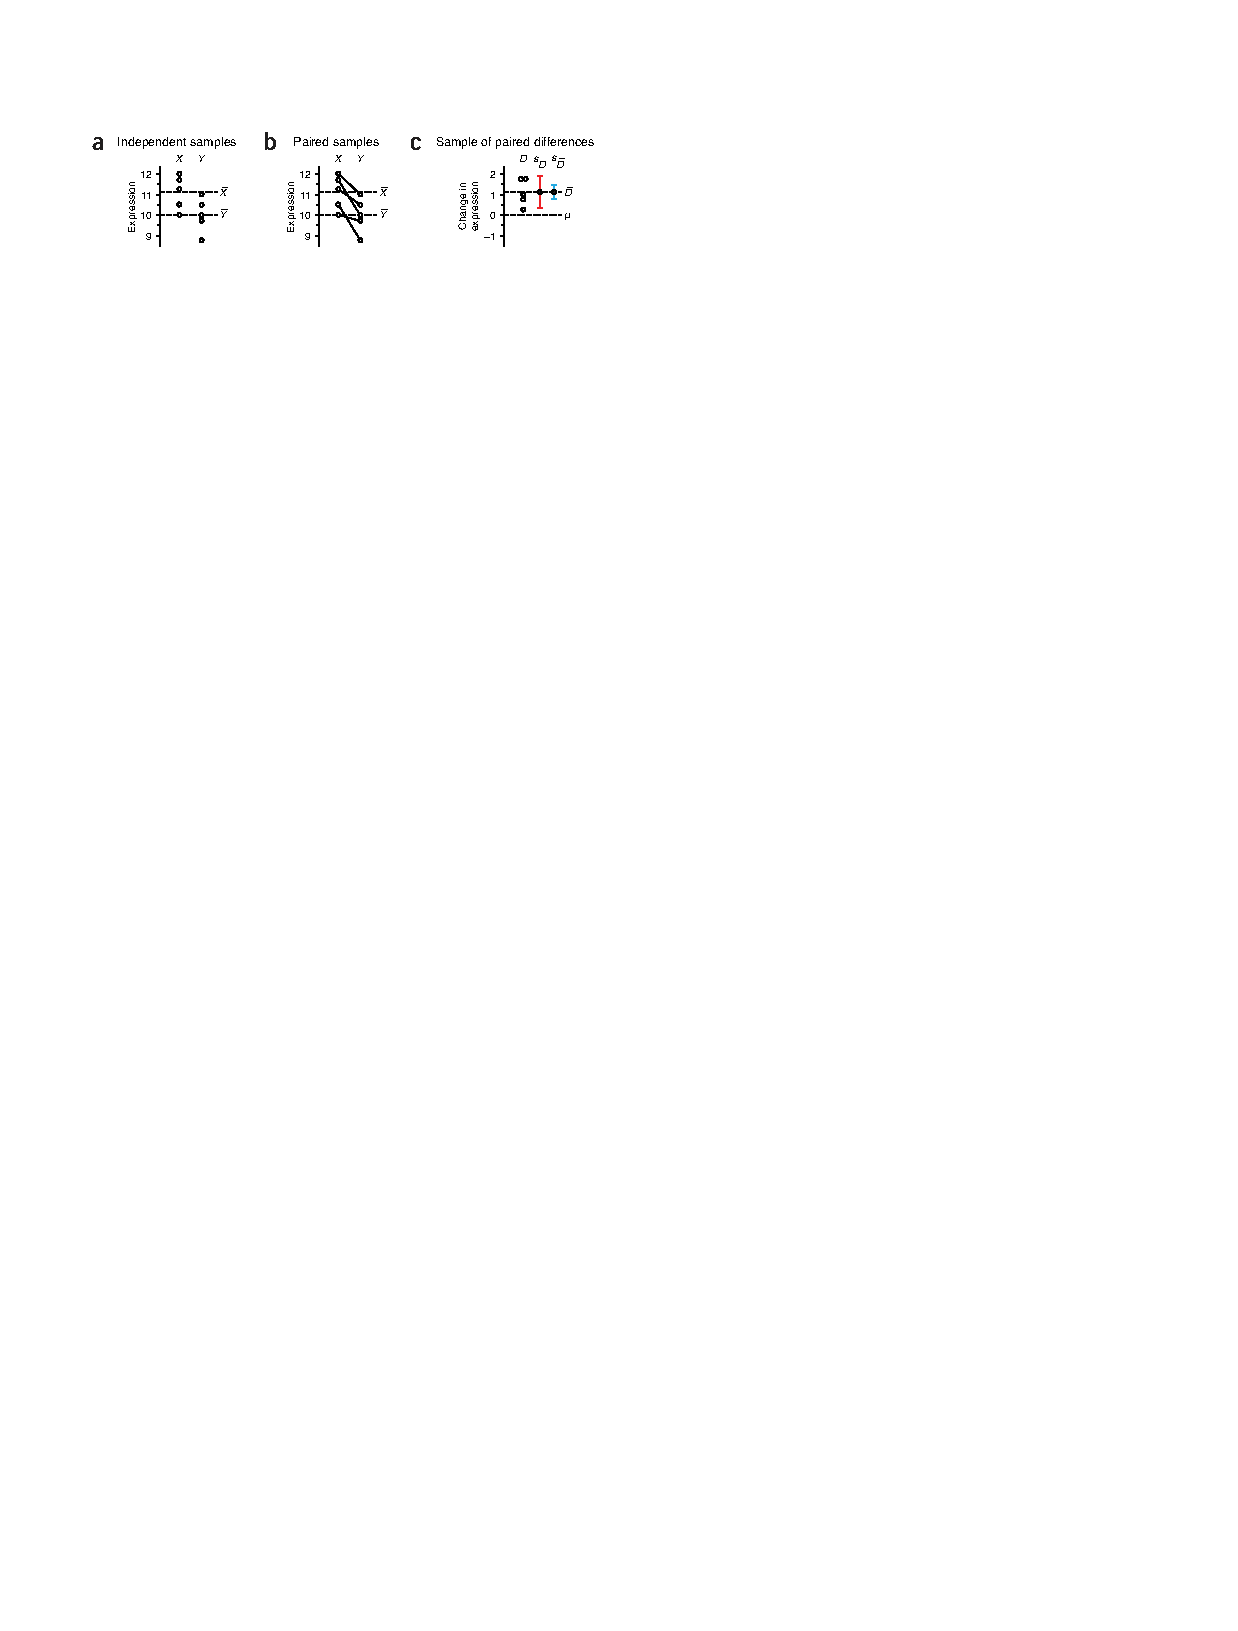
\includegraphics[width=0.98\textwidth]{fig-paired-ttest.pdf}
\end{center}

\credit{Image credit: Krzywinski \& Altman 2014}
\end{frame}

\begin{frame}[fragile,label={sec:org1aef768}]{Paired t-test, example}
 You measure the expression of the gene YFG1 in five mice.  You then treat those five mice with drug X and measure gene expression again.

\begin{itemize}
\item YFG1 expression before treatment = \{11, 10, 10.5, 8.87, 9.75\}
\item YFG1 expression after treatment = \{12, 11.75, 11.25, 10.5, 10\}
\end{itemize}

This data set is available as \texttt{gene-expression-paired.csv} from the course wiki.
\end{frame}

\begin{frame}[fragile,label={sec:org418bda3}]{Hands-on, paired t-test in R}
 \begin{enumerate}
\item Use the \texttt{t.test} function to carry out a paired t-test for paired gene expression data set.
\item Compare your results to the two-sample t-test for the same data if you treat it as unpaired. How do the results differ?  Can you provide an intuitive explanation for why you would get different results when treating the data as paired vs unpaired?
\end{enumerate}
\end{frame}
\end{document}